%%
%% Automatically generated file from DocOnce source
%% (https://github.com/hplgit/doconce/)
%%

% #define PREAMBLE

% #ifdef PREAMBLE
%-------------------- begin preamble ----------------------

\documentclass[%
oneside,                 % oneside: electronic viewing, twoside: printing
final,                   % draft: marks overfull hboxes, figures with paths
10pt]{article}

\listfiles               %  print all files needed to compile this document

\usepackage{relsize,makeidx,color,setspace,amsmath,amsfonts,amssymb}
\usepackage[table]{xcolor}
\usepackage{bm,ltablex,microtype}

\usepackage[pdftex]{graphicx}

\usepackage[T1]{fontenc}
%\usepackage[latin1]{inputenc}
\usepackage{ucs}
\usepackage[utf8x]{inputenc}

\usepackage{lmodern}         % Latin Modern fonts derived from Computer Modern

% Hyperlinks in PDF:
\definecolor{linkcolor}{rgb}{0,0,0.4}
\usepackage{hyperref}
\hypersetup{
    breaklinks=true,
    colorlinks=true,
    linkcolor=linkcolor,
    urlcolor=linkcolor,
    citecolor=black,
    filecolor=black,
    %filecolor=blue,
    pdfmenubar=true,
    pdftoolbar=true,
    bookmarksdepth=3   % Uncomment (and tweak) for PDF bookmarks with more levels than the TOC
    }
%\hyperbaseurl{}   % hyperlinks are relative to this root

\setcounter{tocdepth}{2}  % levels in table of contents

% Tricks for having figures close to where they are defined:
% 1. define less restrictive rules for where to put figures
\setcounter{topnumber}{2}
\setcounter{bottomnumber}{2}
\setcounter{totalnumber}{4}
\renewcommand{\topfraction}{0.95}
\renewcommand{\bottomfraction}{0.95}
\renewcommand{\textfraction}{0}
\renewcommand{\floatpagefraction}{0.75}
% floatpagefraction must always be less than topfraction!
% 2. ensure all figures are flushed before next section
\usepackage[section]{placeins}
% 3. enable begin{figure}[H] (often leads to ugly pagebreaks)
%\usepackage{float}\restylefloat{figure}

% --- fancyhdr package for fancy headers ---
\usepackage{fancyhdr}
\fancyhf{} % sets both header and footer to nothing
\renewcommand{\headrulewidth}{0pt}
\fancyfoot[LE,RO]{\thepage}
% Ensure copyright on titlepage (article style) and chapter pages (book style)
\fancypagestyle{plain}{
  \fancyhf{}
  \fancyfoot[C]{{\footnotesize \copyright\ 2018-2019, Christian Forssén. Released under CC Attribution-NonCommercial 4.0 license}}
%  \renewcommand{\footrulewidth}{0mm}
  \renewcommand{\headrulewidth}{0mm}
}
% Ensure copyright on titlepages with \thispagestyle{empty}
\fancypagestyle{empty}{
  \fancyhf{}
  \fancyfoot[C]{{\footnotesize \copyright\ 2018-2019, Christian Forssén. Released under CC Attribution-NonCommercial 4.0 license}}
  \renewcommand{\footrulewidth}{0mm}
  \renewcommand{\headrulewidth}{0mm}
}

\pagestyle{fancy}


\usepackage[framemethod=TikZ]{mdframed}

% --- begin definitions of admonition environments ---

% Admonition style "mdfbox" is an oval colored box based on mdframed
% "notice" admon
\definecolor{mdfbox_notice_background}{rgb}{1,1,1}
\newmdenv[
  skipabove=15pt,
  skipbelow=15pt,
  outerlinewidth=0,
  backgroundcolor=mdfbox_notice_background,
  linecolor=black,
  linewidth=2pt,       % frame thickness
  frametitlebackgroundcolor=mdfbox_notice_background,
  frametitlerule=true,
  frametitlefont=\normalfont\bfseries,
  shadow=false,        % frame shadow?
  shadowsize=11pt,
  leftmargin=0,
  rightmargin=0,
  roundcorner=5,
  needspace=0pt,
]{notice_mdfboxmdframed}

\newenvironment{notice_mdfboxadmon}[1][]{
\begin{notice_mdfboxmdframed}[frametitle=#1]
}
{
\end{notice_mdfboxmdframed}
}

% Admonition style "mdfbox" is an oval colored box based on mdframed
% "summary" admon
\definecolor{mdfbox_summary_background}{rgb}{1,1,1}
\newmdenv[
  skipabove=15pt,
  skipbelow=15pt,
  outerlinewidth=0,
  backgroundcolor=mdfbox_summary_background,
  linecolor=black,
  linewidth=2pt,       % frame thickness
  frametitlebackgroundcolor=mdfbox_summary_background,
  frametitlerule=true,
  frametitlefont=\normalfont\bfseries,
  shadow=false,        % frame shadow?
  shadowsize=11pt,
  leftmargin=0,
  rightmargin=0,
  roundcorner=5,
  needspace=0pt,
]{summary_mdfboxmdframed}

\newenvironment{summary_mdfboxadmon}[1][]{
\begin{summary_mdfboxmdframed}[frametitle=#1]
}
{
\end{summary_mdfboxmdframed}
}

% Admonition style "mdfbox" is an oval colored box based on mdframed
% "warning" admon
\definecolor{mdfbox_warning_background}{rgb}{1,1,1}
\newmdenv[
  skipabove=15pt,
  skipbelow=15pt,
  outerlinewidth=0,
  backgroundcolor=mdfbox_warning_background,
  linecolor=black,
  linewidth=2pt,       % frame thickness
  frametitlebackgroundcolor=mdfbox_warning_background,
  frametitlerule=true,
  frametitlefont=\normalfont\bfseries,
  shadow=false,        % frame shadow?
  shadowsize=11pt,
  leftmargin=0,
  rightmargin=0,
  roundcorner=5,
  needspace=0pt,
]{warning_mdfboxmdframed}

\newenvironment{warning_mdfboxadmon}[1][]{
\begin{warning_mdfboxmdframed}[frametitle=#1]
}
{
\end{warning_mdfboxmdframed}
}

% Admonition style "mdfbox" is an oval colored box based on mdframed
% "question" admon
\definecolor{mdfbox_question_background}{rgb}{1,1,1}
\newmdenv[
  skipabove=15pt,
  skipbelow=15pt,
  outerlinewidth=0,
  backgroundcolor=mdfbox_question_background,
  linecolor=black,
  linewidth=2pt,       % frame thickness
  frametitlebackgroundcolor=mdfbox_question_background,
  frametitlerule=true,
  frametitlefont=\normalfont\bfseries,
  shadow=false,        % frame shadow?
  shadowsize=11pt,
  leftmargin=0,
  rightmargin=0,
  roundcorner=5,
  needspace=0pt,
]{question_mdfboxmdframed}

\newenvironment{question_mdfboxadmon}[1][]{
\begin{question_mdfboxmdframed}[frametitle=#1]
}
{
\end{question_mdfboxmdframed}
}

% Admonition style "mdfbox" is an oval colored box based on mdframed
% "block" admon
\definecolor{mdfbox_block_background}{rgb}{1,1,1}
\newmdenv[
  skipabove=15pt,
  skipbelow=15pt,
  outerlinewidth=0,
  backgroundcolor=mdfbox_block_background,
  linecolor=black,
  linewidth=2pt,       % frame thickness
  frametitlebackgroundcolor=mdfbox_block_background,
  frametitlerule=true,
  frametitlefont=\normalfont\bfseries,
  shadow=false,        % frame shadow?
  shadowsize=11pt,
  leftmargin=0,
  rightmargin=0,
  roundcorner=5,
  needspace=0pt,
]{block_mdfboxmdframed}

\newenvironment{block_mdfboxadmon}[1][]{
\begin{block_mdfboxmdframed}[frametitle=#1]
}
{
\end{block_mdfboxmdframed}
}

% --- end of definitions of admonition environments ---

% prevent orhpans and widows
\clubpenalty = 10000
\widowpenalty = 10000

% --- end of standard preamble for documents ---


\usepackage[swedish]{babel}

\raggedbottom
\makeindex
\usepackage[totoc]{idxlayout}   % for index in the toc
\usepackage[nottoc]{tocbibind}  % for references/bibliography in the toc

%-------------------- end preamble ----------------------

\begin{document}

% matching end for #ifdef PREAMBLE
% #endif

\newcommand{\exercisesection}[1]{\subsection*{#1}}

\input{newcommands_keep}

% ------------------- main content ----------------------



% ----------------- title -------------------------

\thispagestyle{empty}

\begin{center}
{\LARGE\bf
\begin{spacing}{1.25}
Learning from data: Bayesian Neural Networks
\end{spacing}
}
\end{center}

% ----------------- author(s) -------------------------

\begin{center}
{\bf Christian Forssén}
\end{center}

    \begin{center}
% List of all institutions:
\centerline{{\small Department of Physics, Chalmers University of Technology, Sweden}}
\end{center}
    
% ----------------- end author(s) -------------------------

% --- begin date ---
\begin{center}
Oct 22, 2019
\end{center}
% --- end date ---

\vspace{1cm}


% !split
\section{Bayesian neural networks}
The introduction part of this lecture is inspired by the chapter \emph{"Learning as Inference"} in the excellent book \href{{http://www.inference.org.uk/mackay/itila/}}{Information Theory, Inference, and Learning Algorithms} by David MacKay.

Some python libraries that are relevant for Bayesian Neural Networks (as part of the general trend towards Probabilistic Programming) are:
\begin{itemize}
\item \href{{https://docs.pymc.io/}}{PyMC3}

\item \href{{https://www.tensorflow.org/probability}}{Tensorflow Probability}

\item \href{{https://keras.io/}}{Keras} (for constructing tensorflow models).

\item \href{{http://edwardlib.org/}}{Edward}
\end{itemize}

\noindent
% !split
\subsection{Basic neural network}
We will consider neurons with a vector of $I$ input signals $\mathbf{x} = \left\{ x^{(i)} \right\}_{i=1}^I$, and an output signal $y(a)$, which is a (often non-linear) function of the \emph{activation}
\[ a = w_0 +  \sum_{i=1}^I w_i x_i, \]
where $\mathbf{w} = \left\{ w_i \right\}_{i=1}^I$ are the weights of the neuron and we have included a bias ($b \equiv w_0$).

The training of the network implies feeding it with training data and finding the sets of weights and biases that minimizes a loss function that has been selected for that particular problem.
Consider, e.g., a classification problem where the single output $y$ of the final network layer is a real number $\in [0,1]$ that indicates the (discrete) probability for input $\mathbf{x}$ belonging to either class $t=1$ or $t=0$:
\begin{align}
p_{t=1} \equiv p(t=1 | w,x) &= y \\
p_{t=0} \equiv p(t=0 | w,x) &= 1-y,
\end{align}
where we have simplified the notation, not using boldface anymore for the arrays $w$ and $x$.
A simple neural network classifier can be trained by minimizing the loss function
\[ C_W(w) = C(w) +  \alpha E_W(w), \]
made up of an error function
\[ C(w) = -\sum_n \left[ t^{(n)} \log ( y(x^{(n)},w)) + (1 - t^{(n)}) \log (1 - y(x^{(n)},w)) \right], \]
where $t^{(n)}$ is the training data, and the regularizer
\[ E_W(w) = \frac{1}{2} \sum_i w_i^2, \]
that is designed to avoid overfitting.
The error function can be interpreted as minus the log likelihood
\[ p(D|w) = \exp\left[ - C(w) \right]. \]
Similarly the regularizer can be interpreted in terms of a log prior probability distribution over the parameters
\[ p(w | \alpha) = \frac{1}{Z_W(\alpha)} \exp \left[ -\alpha E_W \right]. \]
If $E_W$ is quadratic as given above, then the corresponding prior distribution is a Gaussian with variance $\sigma_W^2 = 1/\alpha$ and $1/Z_W = (\alpha/2\pi)^{K/2}$, where $K$ is the number of parameters in $w$.
The objective function $C_W(w)$ then corresponds to the inference of the parameters $w$ given the data
\[ p(w | D, \alpha) = \frac{p(D|w) p(w|\alpha)}{p(D|\alpha)} = \frac{1}{Z_M} \exp [ -C_W(w) ]. \]
The network parameters $w$ that are found by minimizing $C_W(w)$ can be interpreted as the (locally) most probable parameter vector $w^*$. We show the different probability distributions for a typical training sequence in the following figure (reproduced from \href{{http://www.inference.org.uk/mackay/itila/}}{Information Theory, Inference, and Learning Algorithms} by David MacKay)


\begin{figure}[!ht]  % 
  \centerline{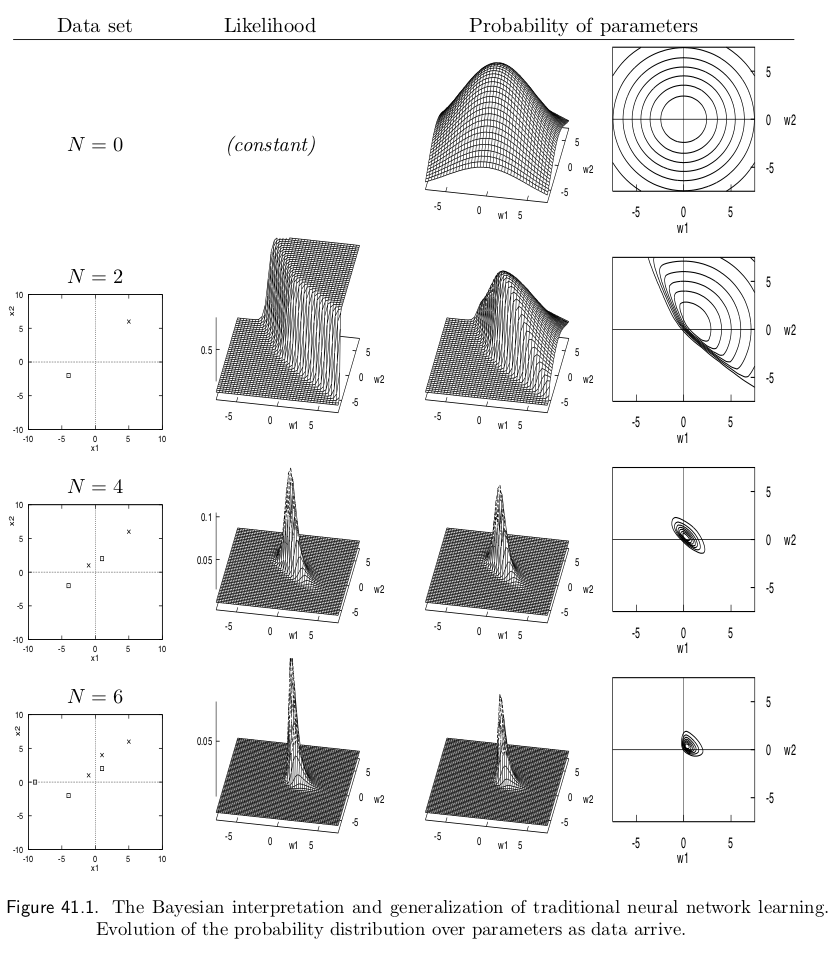
\includegraphics[width=0.8\linewidth]{fig/MacKay_41_1.png}}
  \caption{
  MacKay Fig.~41.1
  }
\end{figure}
%\clearpage % flush figures 


Instead, we will use the Bayesian approach and consider the information that is contained in the probability distribution. 

In fact, there are different uncertainties that should be addressed:

\begin{description}
\item[Epistemic uncertainties:] 
  from uncertainties in the model. For a neural network, this uncertainty can, in principle, be reduced with more data and quantified using the Bayesian approach. Epistemic uncertainty is also known as \textbf{systematic uncertainty}.

\item[Aleatoric uncertainties:] 
  from inherent noise in the training data. This should be included in the likelihood function (and is therefore part of the Bayesian approach). It can, however, not be reduced with more data of the same quality. Aleatoric uncertainty is also known as \textbf{statistical uncertainty}. Aleatoric is derived from the Latin \emph{alea} or dice, referring to a game of chance.
\end{description}

\noindent

\begin{notice_mdfboxadmon}[Notice]
We will use $y$ to denote the output from the neural network. For classification problems, $y$ will give the categorical (discrete) distribution of probabilities $p_{t=c}$ of belonging to class $c$. For regression problems, $y$ is a continuous variable. It could also, in general, be a vector of outputs. The neural network can be seen as a non-linear mapping $y(x; w)$: $x \in \mathbb{R}^p \to y \in \mathbb{R}^m$.
\end{notice_mdfboxadmon} % title: Notice



% !split
\subsection{Probabilistic model}

A Bayesian neural network can be viewed as probabilistic model $p(y \lvert \mathbf{x},\mathbf{w})$. 

Given a training dataset $\mathcal{D} = \left\{\mathbf{x}^{(i)}, y^{(i)}\right\}$ we can construct the likelihood function $p(\mathcal{D} \lvert \mathbf{w}) = \prod_i p(y^{(i)} \lvert \mathbf{x}^{(i)}, \mathbf{w})$ which is a function of parameters $\mathbf{w}$. Maximizing the likelihood function gives the maximimum likelihood estimate (MLE) of $\mathbf{w}$. The usual optimization objective during training is the negative log likelihood. For a categorical distribution this is the \emph{cross entropy} error function, for a Gaussian distribution this is proportional to the \emph{sum of squares} error function. MLE can lead to severe overfitting though.

Multiplying the likelihood with a prior distribution $p(\mathbf{w})$ is, by Bayes theorem, proportional to the posterior distribution $p(\mathbf{w} \lvert \mathcal{D}) \propto p(\mathcal{D} \lvert \mathbf{w}) p(\mathbf{w})$. Maximizing $p(\mathcal{D} \lvert \mathbf{w}) p(\mathbf{w})$ gives the maximum a posteriori (MAP) estimate of $\mathbf{w}$. Computing the MAP estimate has a regularizing effect and can prevent overfitting. The optimization objectives here are the same as for MLE plus a regularization term coming from the log prior.

Both MLE and MAP give point estimates of parameters. If we instead had a full posterior distribution over parameters we could make predictions that take weight uncertainty into account. This is covered by the posterior predictive distribution $p(y \lvert \mathbf{x},\mathcal{D}) = \int p(y \lvert \mathbf{x}, \mathbf{w}) p(\mathbf{w} \lvert \mathcal{D}) d\mathbf{w}$ in which the parameters have been marginalized out. This is equivalent to averaging predictions from an ensemble of neural networks weighted by the posterior probabilities of their parameters $\mathbf{w}$.

Returning to the binary classification problem, $y^{(n+1)}$ corresponds to the probability $p_{t^{(n+1)}=1}$ and a Bayesian prediction of a new datum $y^{(n+1)}$ will correspond to a pdf and involves \emph{marginalizing} over the $K$ weight (and bias) parameters
\[ p(y^{(n+1)} | x^{(n+1)}, D, \alpha) = \int d^K w p( p^{(n+1)} | x^{(n+1)}, w, \alpha) p(w|D,\alpha), \]
where we have also included the weight decay hyperparameter $\alpha$ from the prior (regularizer). Marginalization could, of course, also be performed over this parameter.

We show an example of such inference, comparing the point estimate $y(x; w^*, \alpha)$ and the Bayesian approach, in the follwoing figure (again from MacKay)


\begin{figure}[!ht]  % 
  \centerline{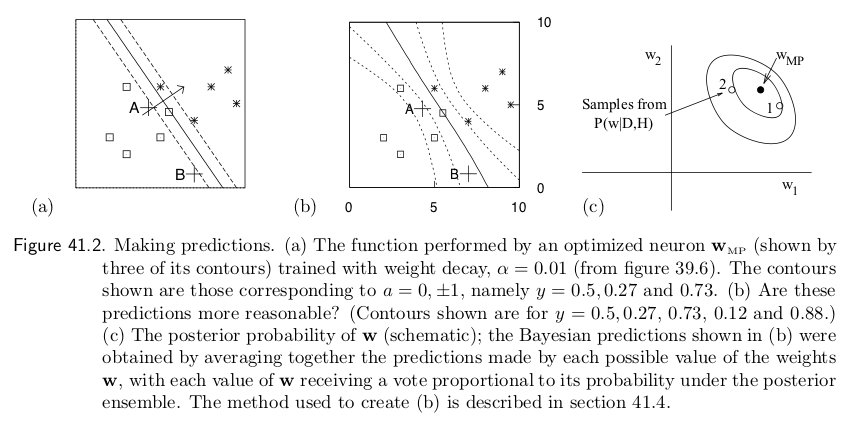
\includegraphics[width=0.8\linewidth]{fig/MacKay_41_2.png}}
  \caption{
  MacKay Fig.~41.2
  }
\end{figure}
%\clearpage % flush figures 


% !split
\subsection{Bayesian neural networks in practice}
But how shall we compute the marginalization integral for serious neural networks with thousands of parameters?

In short, there are three different approaches:

\begin{enumerate}
\item \textbf{Sampling methods}, e.g.~MCMC sampling (this approach would be exact as the number of samples $\rightarrow \infty$);

\item \textbf{Deterministic approximate methods}, for example using Gaussian approximations with the Laplace method;

\item \textbf{Variational methods}.
\end{enumerate}

\noindent
The first two are discussed in MacKay's book, while we will focus on the variational methods in the following.

% !split
\subsection{Variational inference for Bayesian neural networks}

Bayesian neural networks differ from plain neural networks in that their weights are assigned a probability distribution instead of a single value or point estimate. These probability distributions describe the uncertainty in weights and can be used to estimate uncertainty in predictions. Training a Bayesian neural network via variational inference learns the parameters of these distributions instead of the weights directly.

Unfortunately, an analytical solution for the weight posterior $p(\mathbf{w} \lvert \mathcal{D})$ in neural networks is intractable. We therefore have to approximate the true posterior with a variational distribution $q(\mathbf{w} \lvert \boldsymbol{\theta})$ of \textbf{known functional form} whose parameters we want to estimate. 

This can be done by minimizing the \href{{https://en.wikipedia.org/wiki/Kullback%E2%80%93Leibler_divergence}}{Kullback-Leibler divergence} between $q(\mathbf{w} \lvert \boldsymbol{\theta})$ and the true posterior $p(\mathbf{w} \lvert \mathcal{D})$  w.r.t. $\boldsymbol{\theta}$.

The specific goal is then to replace $p(\mathbf{w} \lvert \mathcal{D})$, which we don't know, with the known proxy distribution $q(\mathbf{w} \lvert \boldsymbol{\theta}^*)$, where $\boldsymbol{\theta}^*$ is the optimal set of variational parameters. This optimal set of parameters is typically found by minimizing the \textbf{Evidence Lower Bound} (ELBO), which is equal to the Kullback-Leibler (KL) divergence up to a constant.

% !split
\paragraph{The Kullback-Leibler divergence.}
The KL divergence is a numeric measure of the difference between two distributions. For two probability distributions $q$ and $p$, the KL divergence in a continuous case,
\[ \mathrm{KL}(q||p) = \int_{-\infty}^\infty dx q(x) \log \frac{q(x)}{p(x)} dx \equiv \mathbb{E}_{q(x)} \left[ \log q(x) - \log p(x) \right] \]
As we can see, the KL divergence calculates the expected log differences in between two distributions with respect to distribution q.

Intuitively there are three scenarios:
\begin{itemize}
\item if both $q$ and $p$ are high at the same positions, then we are happy;

\item if $q$ is high where $p$ is low, we pay a price;

\item if $q$ is low we don't care (because of the expectation).
\end{itemize}

\noindent
Note that we could try to reverse these arguments and compute $\mathrm{KL}(p||q)$. However, we choose $\mathrm{KL}(q||p)$ so that we can take expectations.

\paragraph{Variational free energy.}
Using, e.g., Jensen's inequality $f(\mathbb{E}[X]) \ge \mathbb{E}[f(X)]$
it can be shown that the corresponding optimization objective or cost function can be written as

\[ \mathcal{F}(\mathcal{D},\boldsymbol{\theta}) =
\mathrm{KL}(q(\mathbf{w} \lvert \boldsymbol{\theta}) \mid\mid p(\mathbf{w})) -
\mathbb{E}_{q(\mathbf{w} \lvert \boldsymbol{\theta})} \log p(\mathcal{D} \lvert \mathbf{w})
\tag{1} \]
This is known as the \emph{variational free energy}. The first term is the Kullback-Leibler divergence between the variational distribution $q(\mathbf{w} \lvert \boldsymbol{\theta})$ and the prior $p(\mathbf{w})$ and is called the \emph{complexity cost}. The second term is the expected value of the likelihood w.r.t. the variational distribution and is called the \emph{likelihood cost}. By re-arranging the KL term, the cost function can also be written as

\[ \mathcal{F}(\mathcal{D},\boldsymbol{\theta}) =
\mathbb{E}_{q(\mathbf{w} \lvert \boldsymbol{\theta})} \log q(\mathbf{w} \lvert \boldsymbol{\theta}) -
\mathbb{E}_{q(\mathbf{w} \lvert \boldsymbol{\theta})} \log p(\mathbf{w}) -
\mathbb{E}_{q(\mathbf{w} \lvert \boldsymbol{\theta})} \log p(\mathcal{D} \lvert \mathbf{w})
\tag{2} \]
We realize that minimization of the variational free energy is obtained by finding the parameters $\theta$ that
maximizes
\[ \mathbb{E}_{q(\mathbf{w} \lvert \boldsymbol{\theta})} \log \big( p(\mathbf{w}) p(\mathcal{D} \lvert \mathbf{w}) \big) =
\mathbb{E}_{q(\mathbf{w} \lvert \boldsymbol{\theta})} \log p(\mathbf{w, \mathcal{D}}), \]
which encourages weights that fit data well.

and maximizes
\[ - \mathbb{E}_{q(\mathbf{w} \lvert \boldsymbol{\theta})} \log q(\mathbf{w} \lvert \boldsymbol{\theta}) = -\int d \mathbf{w} q(\mathbf{w} \lvert \boldsymbol{\theta}) \log q(\mathbf{w} \lvert \boldsymbol{\theta}), \]
which we recognize as the entropy.

% !split
\subsection{Bayesian neural networks in PyMC3}
In the demonstration notebook of this lecture, it is shown how to use Variational Inference in PyMC3 to fit a simple Bayesian Neural Network. That implementation is based on the \textbf{Automatic Differentation Variational Inference} (ADVI) approach, described e.g.~in \href{{https://arxiv.org/abs/1506.03431}}{Automatic Variational Inference in Stan}.

% !split
\subsection{Bayes by Backprop}

The variational inference approach described in this section is adapted from the \href{{http://krasserm.github.io/2019/03/14/bayesian-neural-networks/}}{blog entry} by Martin Krasser with some modifications. See also the original paper: \href{{https://arxiv.org/abs/1505.05424}}{Weight Uncertainty in Neural Networks} (\emph{Bayes by Backprop}).

We see that all three terms in equation (2) are expectations w.r.t. the variational distribution $q(\mathbf{w} \lvert \boldsymbol{\theta})$. The cost function can therefore be approximated by drawing \href{{https://en.wikipedia.org/wiki/Monte_Carlo_method}}{Monte Carlo} samples $\mathbf{w}^{(i)}$ from $q(\mathbf{w} \lvert \boldsymbol{\theta})$.

\[ \mathcal{F}(\mathcal{D},\boldsymbol{\theta}) \approx {1 \over N} \sum_{i=1}^N \left[
\log q(\mathbf{w}^{(i)} \lvert \boldsymbol{\theta}) -
\log p(\mathbf{w}^{(i)}) -
\log p(\mathcal{D} \lvert \mathbf{w}^{(i)})\right]
\tag{3} \]

In this example, we'll use a Gaussian distribution for the variational posterior, parameterized by $\boldsymbol{\theta} = (\boldsymbol{\mu}, \boldsymbol{\sigma})$ where $\boldsymbol{\mu}$ is the mean vector of the distribution and $\boldsymbol{\sigma}$ the standard deviation vector. The elements of $\boldsymbol{\sigma}$ are the elements of a diagonal covariance matrix which means that weights are assumed to be uncorrelated. Instead of parameterizing the neural network with weights $\mathbf{w}$ directly we parameterize it with $\boldsymbol{\mu}$ and $\boldsymbol{\sigma}$ and therefore double the number of parameters compared to a plain neural network.

% !split
\paragraph{Network training.}
A training iteration consists of a forward-pass and and backward-pass. During a forward pass a single sample is drawn from the variational posterior distribution. It is used to evaluate the approximate cost function defined by equation (3). The first two terms of the cost function are data-independent and can be evaluated layer-wise, the last term is data-dependent and is evaluated at the end of the forward-pass. During a backward-pass, gradients of $\boldsymbol{\mu}$ and $\boldsymbol{\sigma}$ are calculated via backpropagation so that their values can be updated by an optimizer.

Since a forward pass involves a stochastic sampling step we have to apply the so-called \emph{re-parameterization trick} for backpropagation to work. The trick is to sample from a parameter-free distribution and then transform the sampled $\boldsymbol{\epsilon}$ with a deterministic function $t(\boldsymbol{\mu}, \boldsymbol{\sigma}, \boldsymbol{\epsilon})$ for which a gradient can be defined. Here, we choose $\boldsymbol{\epsilon}$ to be drawn from a standard normal distribution i.e.~$\boldsymbol{\epsilon} \sim \mathcal{N}(\mathbf{0}, \mathbf{I})$ and the function $t$ is taken to be $t(\boldsymbol{\mu}, \boldsymbol{\sigma}, \boldsymbol{\epsilon}) = \boldsymbol{\mu} + \boldsymbol{\sigma} \odot \boldsymbol{\epsilon}$, i.e., it shifts the sample by mean $\boldsymbol{\mu}$ and scales it with $\boldsymbol{\sigma}$ where $\odot$ is element-wise multiplication.

For numerical stability we will parameterize the network with $\boldsymbol{\rho}$ instead of $\boldsymbol{\sigma}$ directly and transform $\boldsymbol{\rho}$ with the softplus function to obtain $\boldsymbol{\sigma} = \log(1 + \exp(\boldsymbol{\rho}))$. This ensures that $\boldsymbol{\sigma}$ is always positive. As prior, a scale mixture of two Gaussians is used $p(\mathbf{w}) = \pi \mathcal{N}(\mathbf{w} \lvert 0,\sigma_1^2) + (1 - \pi) \mathcal{N}(\mathbf{w} \lvert 0,\sigma_2^2)$ where $\sigma_1$, $\sigma_2$ and $\pi$ are shared parameters. Their values are learned during training (which is in contrast to the paper where a fixed prior is used).
\paragraph{Uncertainty characterization.}
Uncertainty in predictions that arise from the uncertainty in weights is called \href{{https://en.wikipedia.org/wiki/Uncertainty_quantification}}{epistemic uncertainty}. This kind of uncertainty can be reduced if we get more data. Consequently,  epistemic uncertainty is higher in regions of no or little training data and lower in regions of more training data. Epistemic uncertainty is covered by the variational posterior distribution. Uncertainty coming from the inherent noise in training data is an example of \href{{https://en.wikipedia.org/wiki/Uncertainty_quantification}}{aleatoric uncertainty}. It cannot be reduced if we get more data. Aleatoric uncertainty is covered by the probability distribution used to define the likelihood function.

% ------------------- end of main content ---------------

% #ifdef PREAMBLE
\end{document}
% #endif

